\chapter{CCAP Tool}
In this chapter, we describe the proposed CCAP (Collection Class Access oPtimization) tool.
The CCAP tool accepts two files from the user. One is a Rules file and the other is a java application file that may use Collections class so that we can optimize. We define a grammar to write these rules in the rules file so that the CCAP parser will parse those rules according to the defined grammar and gives CCAP-map as output, which contains a set of patterns along with the optimization code to be inserted in place of code matching the pattern. This CCAP-map is used in checking whether the patterns are present in the input program or not. If any of the patterns are present, then we will again use the CCAP-map to replace those patterns with the target code suggested in the corresponding rule. After modifying the code it will give the optimized code as output.

\begin{figure} [h]
    \centering
    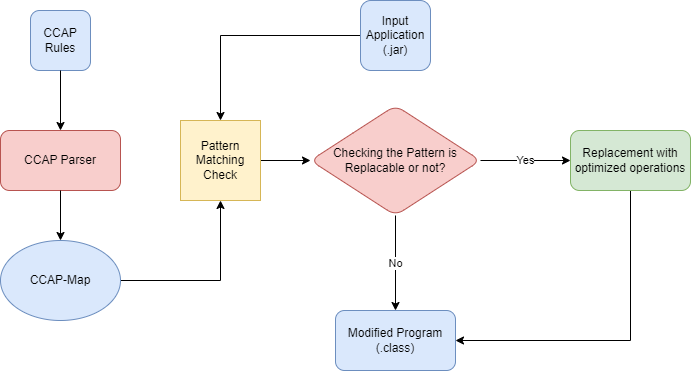
\includegraphics[width = \textwidth]{images/CCAP_tool.png}
    \caption{Workflow of CCAP}
    \label{fig:my_label}
\end{figure}

\section{Rules}
Our goal is to optimize the input program if and only if the program contains certain types of patterns in the code that uses Java collection class methods. The user needs to mention what type of patterns we should replace for optimizing the code and what methods we should use to replace it in the form of Rules. The patterns includes fully qualified method names and initialization statements. These rules will follow a specific format grammar. Only the patterns that are mentioned in these rules will be replaced.


A typical CCAP rule looks like:
\begin{lstlisting} [style = keywords]
Label1:function1(args),Label2:function2(args) {Label1:opfunction1(args)/InitStmt1(args),Label2:opfunctions(args)/InitStmt2(args)} 
\end{lstlisting}

It indicates that , if function1 is called at Label1 and function2 is called at Label2 then replace function 1 with opfunction1/InitStmt1 and function2 with opfunction2/InitStmt2, provided the modified collection of function1 is not used anywhere except label2.

Some sample rules are described below:

\textbf{\small Rules:}

\begin{itemize} [leftmargin=0.5cm]
\item \begin{lstlisting} [style = keywords]
L1:Collections.sort(_,b),L2 : List.get(b,i),{L1:Collections.PriorityQueue(b),L2:PriorityQueue.poll(b)}
\end{lstlisting}
\end{itemize} 

This rule indicates that if there is a Sort method at Label L1 which is expensive and was followed by a cheaper method get at L2 then replace the method at L1 with PriorityQueue and method L2 with poll.\\

\begin{itemize} [leftmargin=0.5cm]
\item \begin{lstlisting} [style = keywords]
L1:Set.retainAll(a,b),L2 : Set.isEmpty(a),{L1:NOP,L2:UserDefined.retainAll_isEmpty(a,b)} 
\end{lstlisting}
\end{itemize}

This rule indicates that if there is Set retainAll method at Label L1 which is expensive and was followed by the cheaper method isEmpty at L2 then replace the method at L1 with NOP, which means there is no need for the method at L1 and method L2 with a user-defined retainAll\textunderscore isEmpty function.This method,instead of doing the complete intersection, simply returns true if it finds atleast one element during the set\textunderscore intersection computation. We have updated the Java library class with many such optimized functions. Fig 3.2 shows a list of such functions.\\

\begin{itemize} [leftmargin=0.5cm]
\item \begin{lstlisting} [style = keywords]
L1:Collections.reverse(_,a),L2:List.toString(a),{L1:NOP,L2:UserDefined.toreverseString(_,a)}
\end{lstlisting}
\end{itemize}

Indicates that if there is a Reverse method at Label L1 which is expensive and was followed by a cheaper method toString at L2 then replace the method at L1 with None and method L2 with a user-defined toReverseString method.\\

\begin{itemize} [leftmargin=0.5cm]
\item \begin{lstlisting} [style = keywords]
L1:List.addAll(a,b),L2:List.toString(a),{L1:NOP,L2:UserDefined.toaddAllString(a,b)}
\end{lstlisting}
\end{itemize}

Indicates that if there is an addAll method at Label L1 which is expensive and was followed by cheaper method toString at L2 then replace the method at L1 with None and method L2 with a user-defined toaddAllString method.\\

\begin{itemize} [leftmargin=0.5cm]
\item \begin{lstlisting} [style = keywords]
L1:List.addAll(a,b),L2:List.toArray(a),{L1:NOP,L2:UserDefined.toaddAllArray(a,b)}
\end{lstlisting}
\end{itemize}

Indicates that if there is an addAll method at Label L1 which is expensive and was followed by a cheaper method toArray at L2 then replace the method at L1 with None and method L2 with user-defined toaddAllArray.\\

\begin{itemize} [leftmargin=0.5cm]
\item \begin{lstlisting} [style = keywords]
L1:List.addAll(a,b),L2:List.contains(a,e),{L1:NOP,L2:UserDefined.contains(a,b,e)}
\end{lstlisting}
\end{itemize}

Indicates that if there is an addAll method at Label L1 which is expensive and was followed by a cheaper method contains at L2 then replace the method at L1 with None and method L2 with user-defined contains.


In these rules the first argument inside the functions represents the base object. if there is no base object then we just use a "\textunderscore" \space as the argument.

\begin{tabular}{ |p{2cm}|p{3cm}|p{8cm}|  }
\hline
%\multicolumn{3}{|c|}{MicroBenchmark Evaluation} \\
Class Name & New function & Description \\
\hline
Set & retainAll\textunderscore isEmpty & returns true immediately after finding a common element between two sets. false otherwise  \\
\hline
List & addAllContains & returns true immediately if required element was found in any of the given lists. false otherwise \\
\hline
List & addAllString & returns string(List format) containing elements from two lists without actually appending the lists \\
\hline
List & addAllArray & returns Array containing elements from two lists without actually appending the lists \\
\hline
Collections  &reverseString & returns string (List format) which is reverse of original without actually reversing the list\\
\hline
\end{tabular}

\begin{figure} [h]
    \centering
    %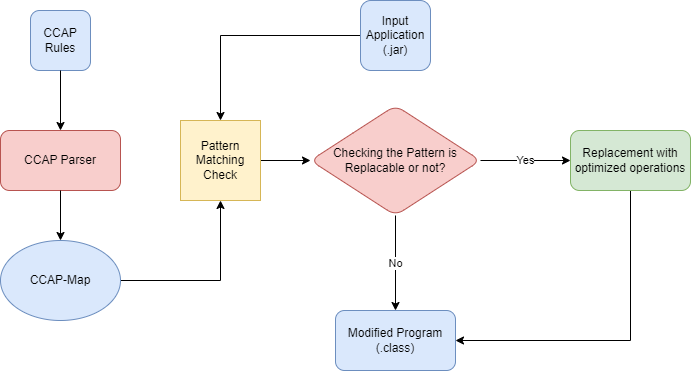
\includegraphics[width = \textwidth]{images/CCAP_tool.png}
    \caption{List of Optimized functions updated to the Java library}
    \label{fig:my_label}
\end{figure}

\section{Parser}
A parser is written using JavaCC and JTB to validate the above mentioned rules and generate the CCAP-map. All the rules follow the below mentioned grammar.

\begin{verbatim}
S -> (Rules)* EOF
Rules -> Label ":" FullName SEPERATOR Label":"FullName SEPERATOR Actions
FullName -> ClassName Stmt | NOP
Stmt -> "." Function "(" Args? ")" | "@" ID "(" Args ")"
ClassName->RESERVED 
Actions->"{" (Action SEPERATOR)+ "}" 
Action -> LabAction | "ForEach" LabAction
LabAction->Label":"FullName
Label->ID
Args->(STRING|NUMBER|"#"|FullName|ID) (RemainingArgs)? 
RemainingArgs -> (STRING|NUMBER|"#"|FullName|ID) (RemainingArgs)?
Function->ID|RESERVED
\end{verbatim}

the keywords in the above grammar represent tokens. which are

\begin{lstlisting} [style = keywords]
    "RESERVED" represents all the fixed class names presented in the collection class like "collections,list,ArrayList" etc
    "ID" represents a identifier which means it can either start with a letter or $ or _ and does not contain any special characters.
    "SEPERATOR" represents a comma(,). used in multiple instances in the rules.
    "NUMBER" represents a numerical value. used as arguments
    "EOF" represents the ending of the file.
\end{lstlisting}

Besides these rules, we will also skip some characters like white spaces, tabs, newlines, etc.

This grammar was written in javacc format and we generated a syntax tree using JavaCC and JTB. Using the visitors generated by JTB we traverse the input rules and store important functions in a data structure called CCAP-Map.

\section{CCAP-map}
This CCAP-Map is a muted hashmap in which the outside map has all the expensive operations as keys and the inside hashmap has cheaper functions as keys. The inner hashmap contains a pair as the value in which the "Pair.method1" represents the replacement for the expensive function and "Pair.method2" contains a replacement for the cheaper function.

 We used hashmap inside another hashmap because it is helpful to run the "Followup tool" on the expensive function, which we will do by directly iterating over all the keys of the hashmap.

 The general format of CCAP-map is 
 \begin{lstlisting} [style = keywords]
     HashMap <String,HashMap <String,Pair>> CCAP_Map
 \end{lstlisting}
 and pair contains 
 \begin{lstlisting} [style= java]
     class Pair{
        List<Object>pair;
        public Pair(Func m1,Func m2)
        {
           this.pair.add(m1);
           this.pair.add(m2);
        }
        public void add(Func m)
        {
            this.pair.add(m);
        }
        public void add(InitStmt i)
        {
            this.pair.add(i);
        }
        public Object get(int i)
        {
            return this.pair.get(i);
        }
     }
     
 \end{lstlisting}

 This "Pair" contains an ArrayList of objects in which we will add either "Func" type object (which corresponds to Function full name) or "InitStmt" type object (which corresponds to Initialization statement). both "Func" and "InitStmt" will contain arguments as a list of ArrayLists as mentioned below.

\begin{lstlisting} [style= java]
    class Func {
        public String func_name;
        public ArrayList<FuncArgs>args;
    }
    class InitStmt {
        public String class_name;
        public String var_name;
        public ArrayList<ArrayList<Integer>>args = new ArrayList<ArrayList<Integer>>();  //constructor arguments
    }
     
 \end{lstlisting}
 
Here each inner ArrayList in "args" contains two integers in which first one is referring to the either of the methods in orginal pattern and second integer reffers to argument index in that method.

For the rules described in chapter 3.1, the CCAP-Map entries are listed below:

\begin{enumerate} [blt]
    \item \begin{lstlisting} [style = keywords]
     CCAP_MAP["Collections.sort"]["List.get"] = (InitStmt("Collections.PriorityQueue",[[0,1]]),Func("PriorityQueue.poll",[])) \end{lstlisting}
     
     \item \begin{lstlisting} [style = keywords]
     CCAP_MAP["Set.retainAll"]["Set.isEmpty"] = ("NOP",Func("UserDefined.retainAll_isEmpty",[[1,0],[0,1]])) \end{lstlisting}
     
     \item \begin{lstlisting} [style = keywords]
     CCAP_MAP["Collections.reverse"]["List.toString"] = ("NOP",Func("UserDefined.toreverseString",[[1,0]])) \end{lstlisting}
     
     \item \begin{lstlisting} [style = keywords]
      CCAP_MAP["List.addAll"]["List.toString"] = ("NOP",Func("UserDefined.toaddAllString",[[1,0],[0,1]])) \end{lstlisting}
      
     \item \begin{lstlisting} [style = keywords]
     CCAP_MAP["List.addAll"]["List.toArray"] = ("NOP",Func("UserDefined.toaddAllArray",[[1,0],[0,1]])) \end{lstlisting}
     
     \item \begin{lstlisting} [style = keywords]
     CCAP_MAP["List.addAll"]["List.contains"] = ("NOP",Func("UserDefined.contains",[[1,0],[0,1],[1,1]])) \end{lstlisting}

\end{enumerate}

For the outer hashmap, the 4 expensive functions act as a hashmap, and these 4 keys again contain different hashmaps with different numbers of keys as shown above.

\section{Algorithm for tool}
The main algorithm for the CCAP tool follows 3 steps. The first step is to generate CCAP-map by reading the rules file from the user with the help of CCAP-Parser. In the next step, we will give this CCAP-Map to the updated followup-tool.

\begin{algorithm} 
\caption{Algorithm for CCAP}\label{alg:cap}
\begin{algorithmic}
\State Mp $\gets$ CCAP\_Map  %\Comment{Initialization of CCAP-Map}

\State Mp $\gets$ CCAP\_Parser(Rule) %\Comment{passing Rules file to CCAP\textunderscore Parser as in Fig 3.1 }
\State Followup\_Function(Mp,InputFile)

\end{algorithmic}
\end{algorithm}

In old followup tool for given function name we find out the followup methods for that function. We extended the function such that we will iterate over all the expensive functions, pass each expensive function name as input to the followup tool. If the obtained followup methods are present in the Hashmap value for the expensive function, then we can say there is a pattern found and we will start generating corresponding replacement units according to the CCAPMap.


\begin{algorithm} 
\caption{Pattern Finding and Replacement Algorithm (Followup tool extension)}\label{alg:Epg}
\begin{algorithmic}
\State entry\_points\_map $\gets$ new HashMap()

\For {each key func\_name in CCAPMap}
\For {each class C}
    \For {each method M in C}
        \For {each followup stmt of func\_name in M}
            \If{stmt contains fc \&\& fc $\in$ CCAPMp[func\_name]}
                \State entry\_points\_map[stmt] $\gets$ Transform(stmt,func\_name)
                \State entry\_points\_map[func\_name] $\gets$ Transform(stmt,func\_name)
            \EndIf
    %\State Mp $\gets$ (val)
         \EndFor
        \EndFor
    \EndFor
\EndFor
\For {each class C}
    \For {each method M in C}
        \For {each key in entry\_points\_map}
            \If{key in M}
                \State swap (key, entry\_points\_map[key])
            \EndIf
    %\State Mp $\gets$ (val)
         \EndFor
        \EndFor
        \State generate modified output file
    \EndFor

\end{algorithmic}
\end{algorithm}

The Pattern Finding and Replacement algorithm presented above is designed as a part of extension to the followup tool. The algorithm works by first creating an entry points map which will store the statements that contain the expensive functions and their corresponding transformed statements. 

The algorithm then iterates over all the expensive functions in the CCAPMap and looks for followup methods in the code. If a followup method is found that contains the expensive function, the algorithm will mark it as an entry point in the entry points map and store the transformed statement using the Transform function. Once all the followup methods containing the expensive functions have been identified, the algorithm iterates over all the methods in the code and checks if any of the entry points are present in the method. If an entry point is found, the algorithm swaps it with its corresponding transformed statement from the entry points map.


While replacing we need to check whether the current pattern is clean or not. It means we need to check the objects affected by the replacement of functions shouldn't be modified/used elsewhere.
%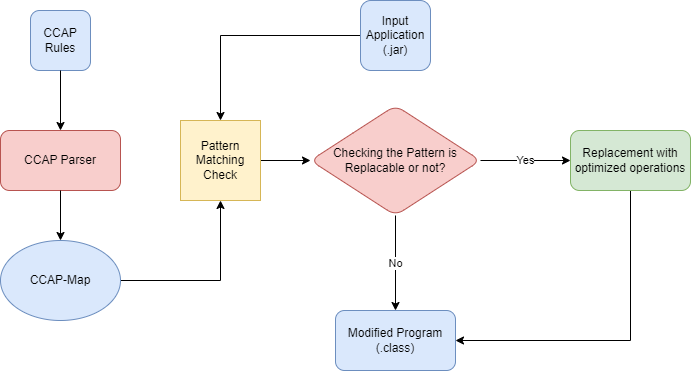
\includegraphics[width=\textwidth]{images/CCAP_tool.png}
